\documentclass[conference]{IEEEtran}
\IEEEoverridecommandlockouts
% The preceding line is only needed to identify funding in the first footnote. If that is unneeded, please comment it out.
\usepackage{cite}
\usepackage{amsmath,amssymb,amsfonts}
\usepackage{algorithmic}
\usepackage{graphicx}
\usepackage{textcomp}
\usepackage{xcolor}
\usepackage[brazilian]{babel}
\usepackage[utf8]{inputenc}
\usepackage[T1]{fontenc}
\usepackage{listings}
\usepackage{color}
\usepackage{float}
\usepackage{multirow}

\definecolor{dkgreen}{rgb}{0,0.6,0}
\definecolor{gray}{rgb}{0.5,0.5,0.5}
\definecolor{mauve}{rgb}{0.58,0,0.82}

\lstset{frame=tb,
  language=Java,
  aboveskip=3mm,
  belowskip=3mm,
  showstringspaces=false,
  columns=flexible,
  basicstyle={\small\ttfamily},
  numbers=none,
  numberstyle=\tiny\color{gray},
  keywordstyle=\color{blue},
  commentstyle=\color{dkgreen},
  stringstyle=\color{mauve},
  breaklines=true,
  breakatwhitespace=true,
  tabsize=3
}
\lstset{language=Python}
\def\BibTeX{{\rm B\kern-.05em{\sc i\kern-.025em b}\kern-.08em
    T\kern-.1667em\lower.7ex\hbox{E}\kern-.125emX}}
\begin{document}

\title{Relatório do Laboratório 5: \\ Estratégias Evolutivas\\
}

\author{\IEEEauthorblockN{Isabelle Ferreira de Oliveira}
\IEEEauthorblockA{\textit{CT-213 - Engenharia da Computação 2020} \\
\textit{Instituto Tecnológico de Aeronáutica (ITA)}\\
São José dos Campos, Brasil \\
isabelle.ferreira3000@gmail.com}
}

\maketitle

\begin{abstract}
Esse relatório documenta a implementação de uma estratégia evolutiva simples e comparação de seu desempenho com o de CMA-ES em funções usadas como \textit{benchmark} para algoritmos de otimização. Essas funções utilizadas eram uma esfera transladada, e as fuções de Ackley, Schaffer 2 e Rastrigin 2D.
\end{abstract}

\begin{IEEEkeywords}
Estratégias evolutivas, CMA-ES, \textit{benchmark}, Ackley, Schaffer 2, Rastrigin 2D
\end{IEEEkeywords}

\section{Introdução}
Otimização consiste em encontrar o mínimo (ou máximo) de uma função, ou seja, encontrar o conjunto de parâmetros que levem essa função ao seu mínimo (ou máximo). Também pode ser visto como encontrar a melhor solução dentre todas as soluções viáveis. Nesses problemas de otimização também é possível haver restrições acerca dos parâmetros que serão analisados.

Dentre os mais diversos tipos de algoritmos de otimização, existem os métodos baseado em estratégias evolutivas, métodos esses inspirados na evolução natural das espécies. Esses métodos seguem a ideia de: dada uma população de possíveis soluções, aplica-se uma função para medir a qualidade dessas soluções candidatas. Essa qualidade quantitativa é chamade de \textit{fitness}. Com base no \textit{fitness}, é possível escolher as melhores soluções e, a partir delas, gerar mutações para se criar uma nova população. Esse processo é repetido até que a convergência chegue a um resultado satisfatório de otimização.

O pseudo-código geral de algortimos utilizando estratégias evolutivas pode ser visto a seguir. Em seguida, será apresentado como esse algoritmo foi implementado no contexto do laboratório.

\begin{lstlisting}
def evolution_strategy(J, m0, C0, hyperparams):
	mu, lambda = unwrap_hyperparams(hyperparams)
	m, C = m0, C0
	while not check_stopping_condition():
		population = multivariate_normal(m, C, lambda)
		population = sort_ascending(population, J)
		parents = population[0:mu]
		m = mean(parents)
	return population[0]
\end{lstlisting}

No pseudocódigo acima, \textit{J} é a função para medir a qualidade das soluções candidatas; \textit{m0} e \textit{C0} são a média e a matriz de covariância iniciais da população que será gerada, respectivamente; \textit{m} e \textit{C} são, de forma análoga, a média e a matriz de covariância atuais da população que será gerada, respectivamente; e \textit{mu} é o tamanho da população considerada como "melhores soluções até então".

\section{Implementação do algoritmo}
Na parte relativa a implementação do algoritmo utilizando uma simples estratégia evolutiva (SES, do inglês \textit{Simple Evolution Strategy}), era necessário preencher a função \textit{tell()} da classe \textit{SimpleEvolutionStrategy}. Recebendo os valores de \textit{fitness} encontrados na população anterior, essa função era a responsável por atualizar a média e a matriz de covariância utilizando os melhores avaliados na antiga população e também evoluir a própria população a cada iteração. Essa função a se completar estava no código base fornecido \cite{b1}.  

Além disso, era necessário comparar os desempenhos desse algoritmo SES com o algoritmo CMA-ES, já fornecido no código base, aplicando-os na otimização de quatro funções, a se saber: esfera transladada, e as fuções de Ackley, Schaffer 2 e Rastrigin 2D.

A análise de vários pontos do algoritmo descrito acima terá uma breve descrição em alto nível da sua implementação a seguir. 

Primeiramente, foi necessário ordenar a população atual tendo em vista os valores de \textit{fitness} associados a ela recebido por parâmetro. Isso foi feito utilizando a função \textit{argsort()} da biblioteca \textit{Numpy}, conforme sugerido pelo roteiro do labotarório.

Após isso, as \textit{mu} melhores amostras dessa população foram separadas para ajudar no cálculo de sua matriz de covariância e, posteriormente, realizar o cálculo da nova média das melhores amostras dessa geração em questão. Essa matriz de covariância foi feita a partir da multiplicação de uma determinada matriz auxiliar pela sua transposta, sendo essa matriz auxiliar a diferença entre essas melhores amostras e a média encontrada na população anterior.

Dessa forma, tendo em posse a nova matriz de covariância e a nova média das melhores amostras da população anterior, é possível gerar uma nova população, evoluindo para a próxima geração de possíveis candidatas a solução.

Para testar o funcionamento dessa implementação, foram alterados os valores das variáveis \textit{algorithm} (entre "ses" e "cmaes") e \textit{function} (entre as funções \textit{translated\underline{\space}sphere}, \textit{ackley}, \textit{schaffer2d}, \textit{rastrigin}) no arquivo \textit{test\underline{\space}evolution\underline{\space}strategy.py} do código base, gerando imagens dos resultados da otimização de cada uma dessas funções usando a estratégia evolutiva escolhida.

Por fim, a fim de realizar o \textit{benchmark} através de simulações de Monte Carlo para comparar os desempenhos dessa estratégia evolutiva simples e do CMA-ES, foram alterados novamente os valores das variáveis \textit{algorithm} e \textit{function}, dessa vez no arquivo \textit{benchmark\underline{\space}evolution\underline{\space}strategy.py} do código base, gerando dessa vez os gráficos comparativos de rendimento para diferentes situações de SES e CMA-ES. Esses gráficos foram apresentados nas Figuras \ref{translated_sphere/mean_fitness} a \ref{rastrigin/best_fitness}.

\section{Resultados e Conclusões}

\subsection{Teste das Estratégias Evolutivas}

A otimização para testar a implementação foi executada para as quatro funções evolutivas já citadas na seção anterior, cuja equação matemática se encontra no roteiro do laboratório \cite{b1}. Os resultados dessas execuções foram satisfatórios e saíram conforme o esperado, comprovando o correto funcionamento da implementação e a validade da utilização das estratégias evolutivos na otimização de funções. Esses resultados foram apresentados nas Figuras de \ref{translated_sphere/ses} a \ref{rastrigin/cmaes}.

Vale reparar que os resultados de ambas implementações foram bastante equivalentes, com exceção do caso da função Rastrigin, no qual cada algoritmo convergiu em míminos locais diferentes.

\begin{figure}[htbp]
\centering
\centerline{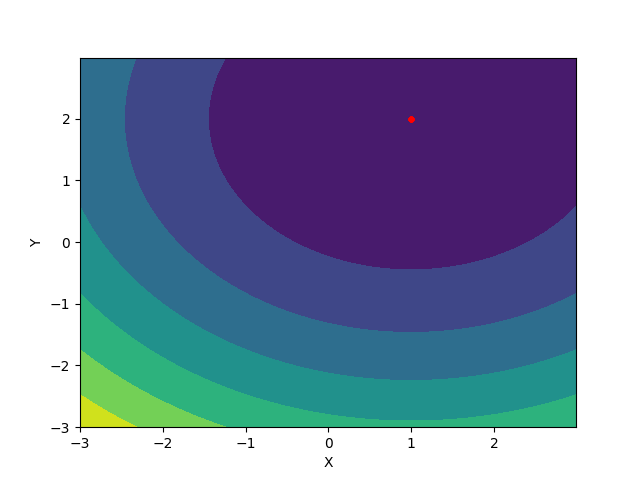
\includegraphics[scale=0.5]{imagens/translated_sphere/ses.png}}
\caption{Otimização da função de Esfera Transladada usando a estratégia evolutiva SES. O resultado encontrado é o ponto vermelho.}
\label{translated_sphere/ses}
\end{figure}

\begin{figure}[htbp]
\centering
\centerline{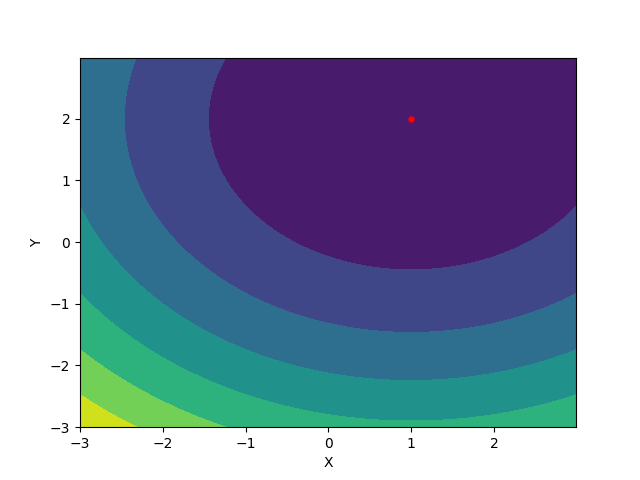
\includegraphics[scale=0.5]{imagens/translated_sphere/cmaes.png}}
\caption{Otimização da função de Esfera Transladada usando a estratégia evolutiva CMA-ES. O resultado encontrado é o ponto vermelho.}
\label{translated_sphere/cmaes}
\end{figure}

\begin{figure}[htbp]
\centering
\centerline{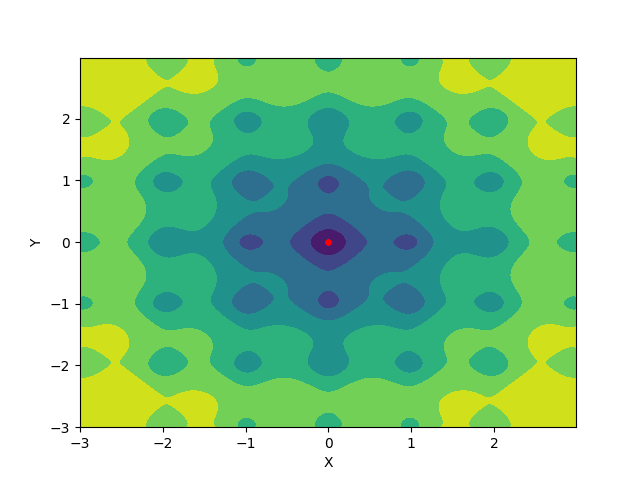
\includegraphics[scale=0.5]{imagens/ackley/ses.png}}
\caption{Otimização da função de Ackley usando a estratégia evolutiva SES. O resultado encontrado é o ponto vermelho.}
\label{ackley/ses}
\end{figure} 

\begin{figure}[htbp]
\centering
\centerline{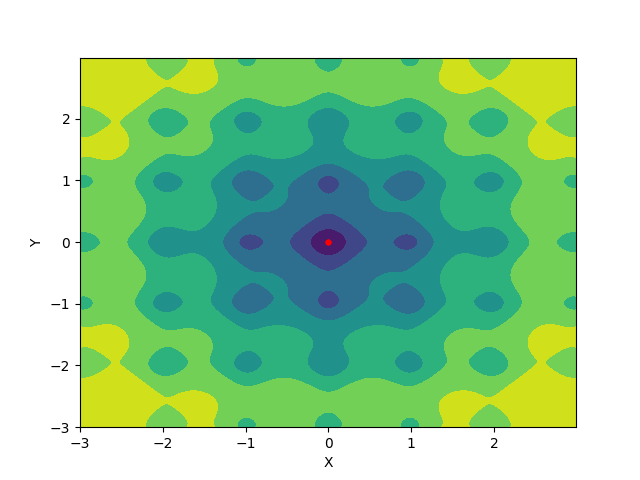
\includegraphics[scale=0.5]{imagens/ackley/cmaes.png}}
\caption{Otimização da função de Ackley usando a estratégia evolutiva CMA-ES. O resultado encontrado é o ponto vermelho.}
\label{ackley/cmaes}
\end{figure}

\begin{figure}[htbp]
\centering
\centerline{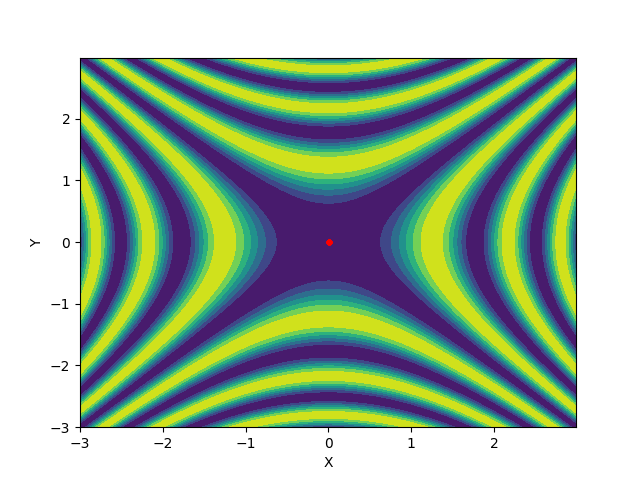
\includegraphics[scale=0.5]{imagens/schaffer2d/ses.png}}
\caption{Otimização da função de Schaffer Nº 2 usando a estratégia evolutiva SES. O resultado encontrado é o ponto vermelho.}
\label{schaffer2d/ses}
\end{figure} 

\begin{figure}[htbp]
\centering
\centerline{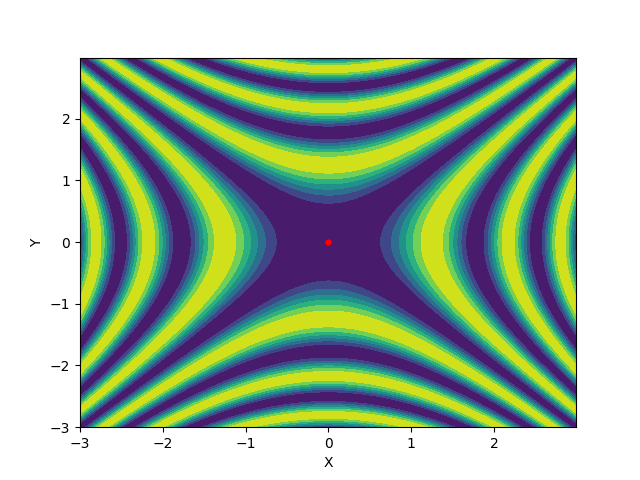
\includegraphics[scale=0.5]{imagens/schaffer2d/cmaes.png}}
\caption{Otimização da função de Schaffer Nº 2 usando a estratégia evolutiva CMA-ES. O resultado encontrado é o ponto vermelho.}
\label{schaffer2d/cmaes}
\end{figure}

\begin{figure}[htbp]
\centering
\centerline{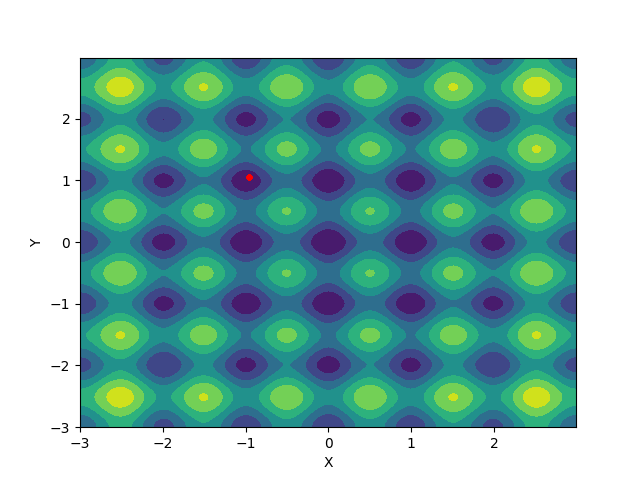
\includegraphics[scale=0.5]{imagens/rastrigin/ses.png}}
\caption{Otimização da função Rastrigin (2D) usando a estratégia evolutiva SES. O resultado encontrado é o ponto vermelho.}
\label{rastrigin/ses}
\end{figure} 

\begin{figure}[htbp]
\centering
\centerline{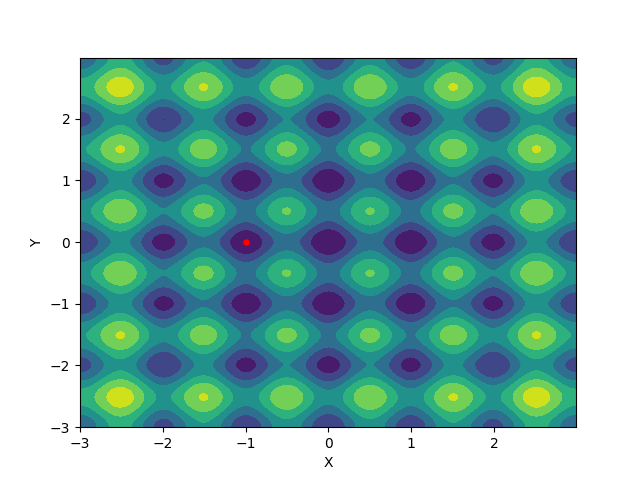
\includegraphics[scale=0.5]{imagens/rastrigin/cmaes.png}}
\caption{Otimização da função Rastrigin (2D) usando a estratégia evolutiva CMA-ES. O resultado encontrado é o ponto vermelho.}
\label{rastrigin/cmaes}
\end{figure}

\subsection{Benchmark das Estratégias Evolutivas}

A otimização para realizar o \textit{benchmark} do desempenho de cada um dos métodos evolutivos estudados (SES e CMA-ES) para diferentes funções e parâmetros foi executada para as quatro funções evolutivas já citadas. Os resultados dessas execuções demonstraram comportamentos coerentes e foram apresentados nas Figuras de \ref{translated_sphere/ses} a \ref{rastrigin/cmaes}.

É possível salientar que, embora sempre tenha havido convergências após um número significativo de iterações, nem todas as convergências chegaram a mínimos locais, como por exemplo para a função da Esfera Transaladada, que só possui um mínimo local (que também é global), mas cada situação testada chegou a valores diferentes de \textit{fitness}.

Além disso, notou-se que, para estratégias evolutivas mais simples, é necessário um número cada vez maior de elementos na população para que os resultados se tornem cada vez mais otimizados. Já para o algoritmo CMA-ES precisou de cerca de 1/4 de população para alcançar resultados similares aos do SES. Isso aconteceu para todos os casos com exceção à função Schaffer Nº 2, que estratégias mais simples e com menores populações se saíram melhor em desempenho do que CMA-ES.

\begin{figure}[htbp]
\centering
\centerline{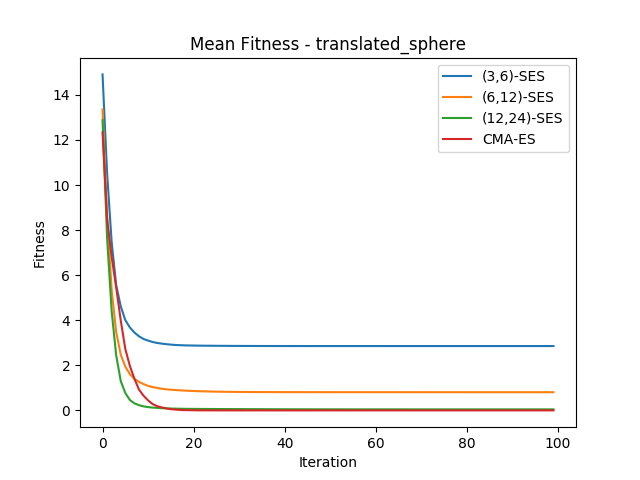
\includegraphics[scale=0.5]{imagens/translated_sphere/mean_fitness.png}}
\caption{Evolução (e convergência) dos valores médios de fitness das populações em cada iteração para diferentes métodos evolutivos e parâmetros para a função Esfera Transladada.}
\label{translated_sphere/mean_fitness}
\end{figure}

\begin{figure}[htbp]
\centering
\centerline{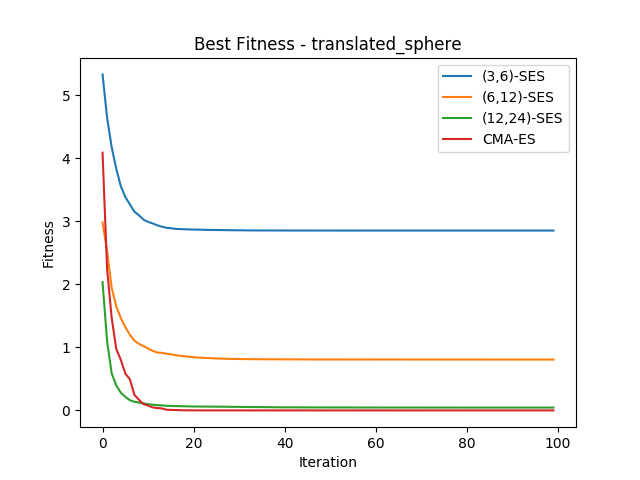
\includegraphics[scale=0.5]{imagens/translated_sphere/best_fitness.png}}
\caption{Evolução (e convergência) dos melhores valores de fitness das populações em cada iteração para diferentes métodos evolutivos e parâmetros para a função Esfera Transladada.}
\label{translated_sphere/best_fitness}
\end{figure}

\begin{figure}[htbp]
\centering
\centerline{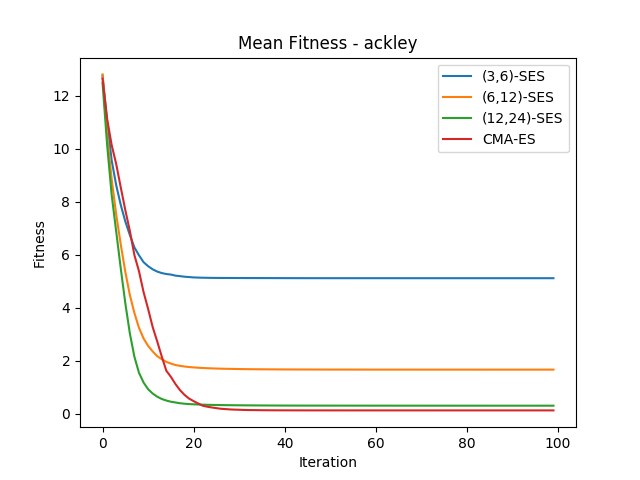
\includegraphics[scale=0.5]{imagens/ackley/mean_fitness.png}}
\caption{Evolução (e convergência) dos valores médios de fitness das populações em cada iteração para diferentes métodos evolutivos e parâmetros para a função Ackley.}
\label{ackley/mean_fitness}
\end{figure}

\begin{figure}[htbp]
\centering
\centerline{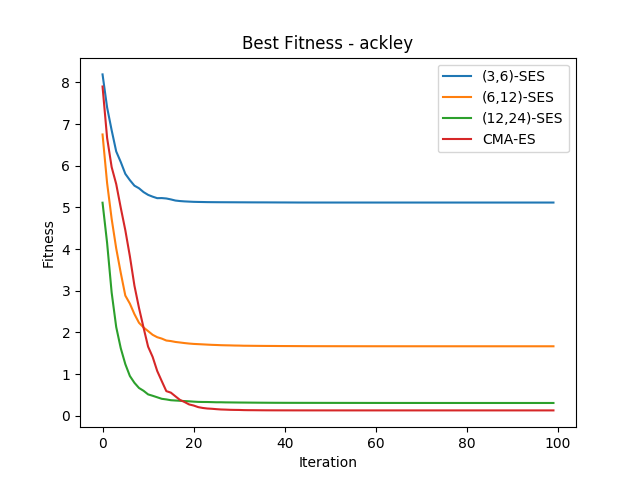
\includegraphics[scale=0.5]{imagens/ackley/best_fitness.png}}
\caption{Evolução (e convergência) dos melhores valores de fitness das populações em cada iteração para diferentes métodos evolutivos e parâmetros para a função Ackley.}
\label{ackley/best_fitness}
\end{figure}

\begin{figure}[htbp]
\centering
\centerline{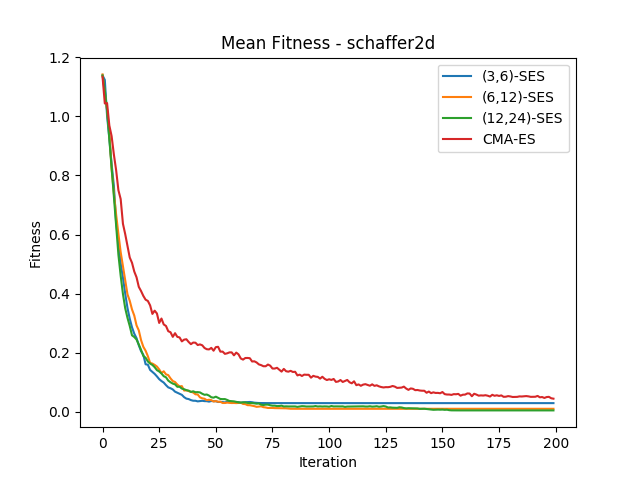
\includegraphics[scale=0.5]{imagens/schaffer2d/mean_fitness.png}}
\caption{Evolução (e convergência) dos valores médios de fitness das populações em cada iteração para diferentes métodos evolutivos e parâmetros para a função Schaffer Nº 2.}
\label{schaffer2d/mean_fitness}
\end{figure}

\begin{figure}[htbp]
\centering
\centerline{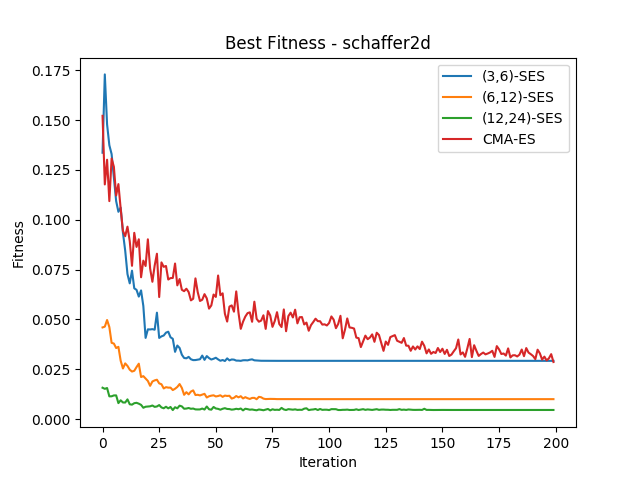
\includegraphics[scale=0.5]{imagens/schaffer2d/best_fitness.png}}
\caption{Evolução (e convergência) dos melhores valores de fitness das populações em cada iteração para diferentes métodos evolutivos e parâmetros para a função Schaffer Nº 2.}
\label{schaffer2d/best_fitness}
\end{figure}

\begin{figure}[htbp]
\centering
\centerline{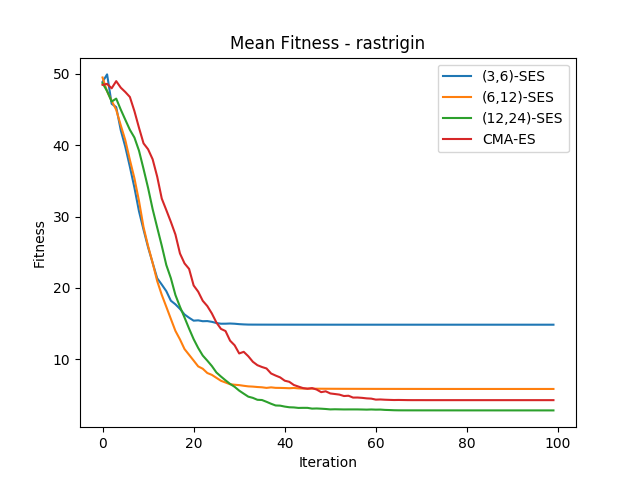
\includegraphics[scale=0.5]{imagens/rastrigin/mean_fitness.png}}
\caption{Evolução (e convergência) dos valores médios de fitness das populações em cada iteração para diferentes métodos evolutivos e parâmetros para a função Rastrigin (2D).}
\label{rastrigin/mean_fitness}
\end{figure}

\begin{figure}[htbp]
\centering
\centerline{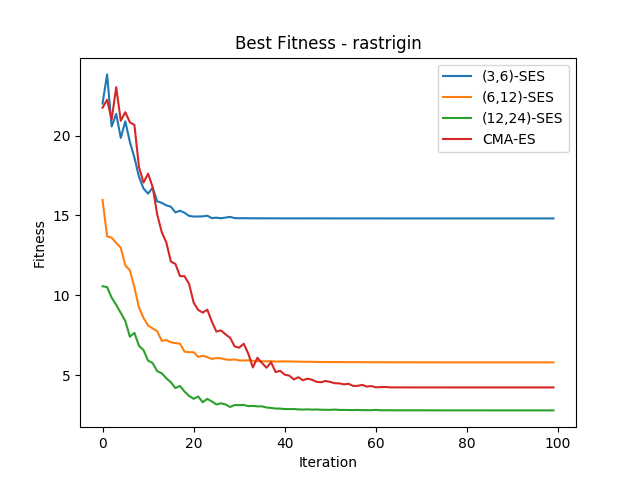
\includegraphics[scale=0.5]{imagens/rastrigin/best_fitness.png}}
\caption{Evolução (e convergência) dos melhores valores de fitness das populações em cada iteração para diferentes métodos evolutivos e parâmetros para a função Rastrigin (2D).}
\label{rastrigin/best_fitness}
\end{figure}

Tendo em vista o que foi apresentado, pode-se notar, por fim, que esses algoritmos realmente se demonstraram eficazes em encontrar parâmetros otimizados para uma determinada função.

\begin{thebibliography}{00}
\bibitem{b1} M. Maximo, ``Roteiro: Laboratório 5 - Estratégias Evolutivas''. Instituto Tecnológico de Aeronáutica, Departamento de Computação. CT-213, 2019.
\end{thebibliography}

\end{document}
